\documentclass[11pt]{article}
\usepackage{hyperref}
\usepackage{common}
\title{HW3 Neural Machine Translation}
\author{Roshan Padaki \\ rpadaki@college.harvard.edu \and Michael Zhang \\ michael\_zhang@college.harvard.edu }
\begin{document}

\maketitle{}
\section{Introduction}

With the advent and advances of data processing, computation, and new algorithms associated with recent developments in deep learning, neural machine translation (NMT) has demonstrated impressive performance. Compared to traditional statistical machine translation, which often relied on handcrafted linguistic rules and probabilistic models, NMT can succeed through an end-to-end training schema through a single neural network.

In this assignment, we explore two NMT models: 1) a baseline sequence-to-sequence model making use of an encoder and decoder LSTM joined together as in \cite{43155}, and 2) an attention-driven deep learning model inspired by \cite{DBLP:journals/corr/BahdanauCB14}. With these, we wish to translate German to English. From an out-of-sample test set of 800 German sentences, we generate 100 of the most probable 3-gram s.

\section{Problem Description}
We aim to perform machine translation as follows. Let $\mathcal{V}_\text{src}$ be our vocabulary of German words, and $\mathcal{V}_\text{trg}$ be our vocabulary of English words. Given a German source sentence of length $S$, which we model as a sequence of words $\mathbf{x} = (x_1, \ldots, x_S)$, we aim to produce a translation $\mathbf{y} = (y_1, \ldots, y_T)$, denoting an English sentence with $T$ not necessarily $= S$ words. 

For the purposes of training and evaluation, we do not use the BLEU score as described in \cite{P02-1040}, but instead rely on perplexity (PPL). For each word with index $i \in [1, T]$ of a target sentence, our network incorporates both the source sentence and the partial translation $y_1, \ldots, y_{i-1}$ to predict word $y_i$, hoping to learn the distribution
\[
p(y_i | \mathbf{x}, y_1, \ldots y_{i-1})
\]
Letting $f$ be the function computed by two recurrent neural networks as standard in the sequence-to-sequence architecture, we train to minimize the expected negative log-likelihood of the correct word $y_i$, reporting perplexity
\[
\text{PPL}(f) = \exp \left\{\frac{1}{T}\sum_{t=1}^T - \ln f(y_t\; \mathbf{x}, y_1, \ldots, y_{t-1}) \right\}
\]
where we make explicit the input parameters of our neural net.


% \begin{center}
%     \begin{tabular}{@{}lll@{}}
%         % \toprule
%         &\multicolumn{2}{c}{} \\
%         & Variable & Definition\\
%         \midrule
%         & $\sigma$ & Activation function (sigmoid, tanh, ReLU) \\
%         & $\boldb$ & Bias term(s) \\
%         & $\bolde$ & Embedding vector \\
%         & $\boldx$ & Word vector \\
%         & $\boldw, p, c$ & Convolutional terms: filter, dropout prob., feature\\
%         & $\mcP, \mcN$ & Training data: positive sentences, negative sentences \\
%         \bottomrule
%     \end{tabular}
% \end{center}


\section{Model and Algorithms}
As mentioned earlier, we implemented and trained two translation model classes: a baseline sequence-to-sequence model, and a modification incorporating attention. For consistency, we refer to indices $s \in \{1, 2, \ldots, S\}$ for our source words, and $t \in \{1, 2, \ldots, T\}$ for the target words.

\subsection{Sequence-to-Sequence (Seq2Seq)}
Our Seq2Seq network consists of an encoder LSTM and a decoder LSTM, each implemented with multiple layers. Given an input sentence $\mathbf{x}$ with length $S$ and embedding layer, the encoder outputs a fixed-length context vector $c$, such that
\[
h_s^e = f(x_s, h_{s-1}^e) \;\; \forall\; s = 1, \ldots, S
\]
\[
c = g(\left{h_1, \ldots, h_S^e\right})
\]
where $h_s^e$ is the hidden state of the encoder with $h_0 = \mathbf{0}$ and $g$ is a function the hidden cells. Ultimately, we feed in the last hidden state $h_S^e$ to the decoder, such that if we denote $h_t^d$ to be the $t$th hidden state of the decoder, we have $h_0^d = h_S^e$. The decoder then produces outputs
\[
\begin{aligned}
z_t = f'(y_t, z_{t-1}) \;\; \forall\; 1, \ldots, T
\end{aligned}
\]
where $y_t$ is the $t$th word of the given partial translation. We then wish to predict the probability distribution of the $t +1$th word in the output, doing so with a softmax function such that our approximating distribution $q$ is given by
\[
q(y_{t+1} | \mathbf{x}, y_1, \ldots, y_{t}) = \text{softmax}(W z_t + b)
\]
where $W$ is a $|\mathcal{V}_\text{trg}| \times n_h$ weight matrix, letting $n_h$ be the hidden layer size of the network, and $b$ being a $n_h$-dimensional bias vector. Here, we model both LSTMs to have the same number of hidden cells.  

\subsection{Attention}
In addition to the vanilla Seq2Seq model described above, we also incorporate attention as described in \cite{DBLP:journals/corr/BahdanauCB14}. Our encoder architecture remains the same to the model without attention, but we also experiment with bidirectionality in our encoding LSTM. Once more, the encoder consists of an embedding layer followed by an $n$-layer LSTM with hidden size $n_h$, and outputs hidden and cell states $(h_s, c_s) \in \mathbb{R}^{n \times n_h}$ for the last word in the input, and outputs $o_s \in \mathbb{R}^{n_h}$ at the last LSTM layer for all words in the input.

The decoder also consists of an embedding layer and an $n$-layer LSTM with hidden size $n_h$, taking in as input the last hidden and cell states of the encoder. With output $o_t \in \mathbb{R}^{n_h}$ being the output of the decoder LSTM, we compute attention at each time-step with
\[
\alpha_t = S(f(o_{1:S}, o_t))
\]
where we have
\[
f = (\textbf{W} o_{1:S} + b) \cdot o_t
\]
which allows us to transform the encoder's output to match that of the decoder. With the attention weights, we can construct context vector $c_t$ such that
\[
c_t = \sum_{s=1}^S \alpha_{t}o_s
\]
and we can calculate the probability distribution over our target English vocab words with
\[
q(y_{t+1} | \textbf{x}, y_{1:t}) = S(\mathbf{W}(o_t, c_t)^\trans + b)
\]

\subsection{Beam Search}
Towards actually generating translations, our decoder outputs vectors of probability over the vocabulary (denoted $p_i \in \mathbb{R}^V$ for vocabulary of size $V$) such that for a given target sequence $y_1, \ldots, y_T$, we can compute the probability as the product of the probabilities of each token at every relevant time step, given by
\[
p(y_1, \ldots, y_T) = \prod_{i=1}^Tp_i(y_i)
\]
letting $p_i(y_i)$ be the $y_i$-th item of the probability vector $p_i$ from the $i$-th decoding step. Towards maximizing the probability of our actual target sequence, we thus seek to minimize the negative log likelihood, given by
\[
-\log p(y_1, \ldots, y_T) = -\sum_{i=1}^T \log p_i(y_i)
\]
However, just feeding in the the best token at each step of our LSTM decoder calculation may propagate smaller stepwise mistakes into larger errors, which thus motivates our beam search algorithm. Now, instead of predicting only the token with the best score, we keep track of $k$ hypotheses, where $k$ is referred to as the beam size. At each time step, for each hypothesis we have $V$ possible tokens, and only select the best $k$ before proceeding. More formally, if $\mathbf{H}_t$ is the set of hypotheses at time step $t$ where
\[
\mathbf{H}_t = \left\{(y_1^1, \ldots y_t^1), (y_1^2, \ldots y_t^2), \ldots, (y_1^k, \ldots y_t^k) \right\}
\]
then we consider all possible candidates $\mathbf{C}_{t+1}$ produced from $\mathbf{H}_t$ by adding new tokens
\[
\mathbf{C}_{t+1} = \bigcup_{i=1}^k \left\{(y_1^i, \ldots y_t^i, 1), \ldots, (y_1^i, \ldots, y_t^i, V )\right\}
\]
we only keep the tokens associated with the $k$ highest scores. When we reach the end-of-sentence token, we then return the hypothesis with the highest score, thus remaining more robust to single token errors.


% Here you specify the model itself. This section should formally
% describe the model used to solve the task proposed in the previous
% section. This section should try to avoid introducing new vocabulary
% or notation, when possible use the notation from the previous section.
% Feel free to use the notation from class, but try to make the note
% understandable as a standalone piece of text.

% This section is also a great place to include other material that
% describes the underlying structure and choices of your model, for
% instance here are some example tables and algorithms from full
% research papers:

% \begin{itemize}
% \item diagrams of your model,

%   \begin{center}
%     \includegraphics[width=0.4\textwidth]{network}
%   \end{center}
% \item feature tables,

%   \begin{center}
%     \begin{tabular}{@{}lll@{}}
%       \toprule
%       &\multicolumn{2}{c}{Mention Features  } \\
%       & Feature & Value Set\\
%       \midrule
%       & Mention Head & $\mcV$ \\
%       & Mention First Word & $\mcV$ \\
%       & Mention Last Word & $\mcV$ \\
%       & Word Preceding Mention & $\mcV$ \\
%       & Word Following Mention & $\mcV$\\
%       & \# Words in Mention & $\{1, 2, \ldots \}$ \\
%       & Mention Type & $\mathcal{T}$ \\
%       \bottomrule
%     \end{tabular}
%   \end{center}

% \item pseudo-code,

%   \begin{algorithmic}[1]
%     \Procedure{Linearize}{$x_1\ldots x_N$, $K$, $g$}
%     \State{$B_0 \gets \langle (\langle \rangle, \{1, \ldots, N\}, 0, \boldh_0, \mathbf{0})  \rangle$}
%     \For{$m = 0, \ldots, M-1$ }
%     \For{$k = 1, \ldots, |B_m|$}
%     \For{$i \in \mcR$}
%     \State{$(y, \mcR, s, \boldh) \gets \mathrm{copy}(B_m^{(k)})$}
%     \For{word $w$ in phrase $x_i$}
%     \State{$y \gets y $ append $w$ }
%     \State{$s \gets s + \log q(w, \boldh) $ }
%     \State{$\boldh \gets \delta(w, \boldh)$}
%     \EndFor{}
%     \State{$B_{m+|w_i|} \gets B_{m+|w_i|} + (y, \mcR - i, s,   \boldh)$}
%     \State{keep top-$K$ of $B_{m+|w_i|}$ by $f(x, y) + g(\mcR)$}
%     \EndFor{}
%     \EndFor{}
%     \EndFor{}
%     \State{\Return{$B_{M}^{(k)}$}}
%     \EndProcedure{}
%   \end{algorithmic}

% \end{itemize}

\section{Experiments}
For all models, we trained with a corpus of 200K sentence German and English sentence pairs, capping our sentence lengths to 20 words. We trained models for 10 epochs, employing early stopping through empirical observation of validation perplexity when appropriate. In addition, for all models we fed in sentences with batch-length $32$, and initiated recurrent model parameters uniformly in the interval $[-0.05, 0.05]$. Table 1 reports our perplexities for our basic Seq2Seq and Seq2Seq with attention models. Towards actual translation output, we implemented beam search as part of evaluation, sticking with a beam size of $100$. \\

\begin{table}[h]
\centering
\begin{tabular}{llr}
 \toprule
 Model &  & Perplexity \\
 \midrule
 \textsc{Vanilla Seq2Seq} & & 8.18\\
 \textsc{Attention Seq2Seq} & & 4.48 \\
 \bottomrule
\end{tabular}
\caption{\label{tab:results} Basic model performance with regard to validation perplexities}
\end{table}

\subsection{Vanilla Seq2Seq}
For our Vanilla Seq2Seq model without attention, we used a standard encoder-decoder LSTM architecture employing two LSTMs each with $500$ nodes per layer. We used $500$-dimensional embeddings as an initial input, and experimented with between 2 and 4 hidden layers. We also considered reversing the input sentence when training as reported in \cite{43155}, however when attempting to do so evidence from early epochs suggested that our validation perplexity would not significantly improve. We hypothesize that this may be due to the fairly short nature of our sentences. Finally, we used stochastic gradient descent (SGD) with regard to optimizing negative log-likelihood (NLL) during training, and as a heuristic employed a decaying learning rate initiated at $0.7$, halving this after every epoch starting at the $5$th epoch.

\subsection{Seq2Seq with Attention}
Given the preliminary results of our Vanilla Seq2Seq model, we sought to characterize the addition of attention. Using the same overall encoder-decoder model architecture, we also employed an initial hidden layer size of $500$ over $4$ hidden layers per encoder and decoder, but found performance boosts widening our net to $650$ hidden nodes per layer. Our encoder was practically unchanged, but our decoder implemented attention utilizing a concatenation of both previous context and decoder output to inform our encoder's output. We employ dropout of $0.2$ on the hidden layers of both the encoder and decoder LSTMs to combat overfitting. Finally we also experiment with weight-tying as presented in \cite{DBLP:journals/corr/PressW16} on grounds of performance boosting in Homework 2. For Kaggle submission, we employed beam search with beam size $100$, achieving a score of $0.338$ and beating the set baseline at $0.238$.

\subsection{Attention Visualization}

With the latter implementation of Seq2Seq with attention, we were able to capture an attention distribution for various sentences, as seen in Figure 1. 

\begin{figure}[htp]
\centering
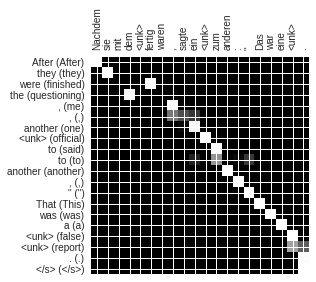
\includegraphics[width=.3\textwidth]{hw3/writeup/img/attn_vis_1.png}
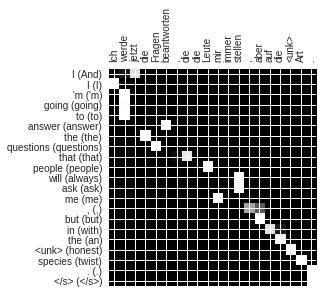
\includegraphics[width=.3\textwidth]{hw3/writeup/img/attn_vis_2.png}
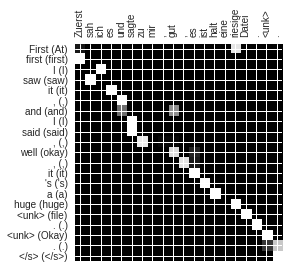
\includegraphics[width=.3\textwidth]{hw3/writeup/img/attn_vis_3.png}

\medskip

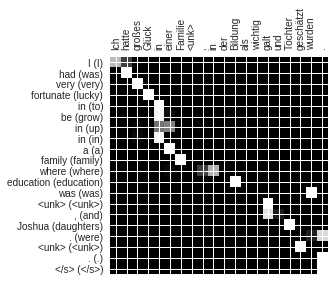
\includegraphics[width=.3\textwidth]{hw3/writeup/img/attn_vis_4.png}
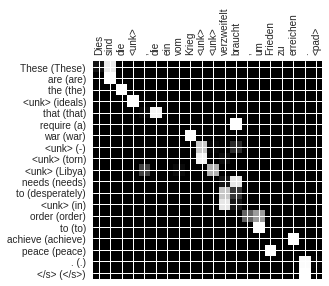
\includegraphics[width=.3\textwidth]{hw3/writeup/img/attn_vis_5.png}
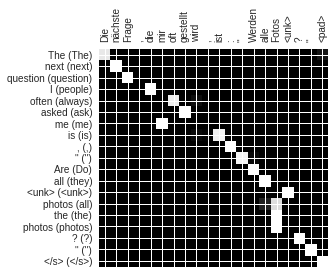
\includegraphics[width=.3\textwidth]{hw3/writeup/img/attn_vis_6.png}

\caption{Example sentence attention distributions. Lighter squares denote higher weights. The x-axis and y-axis of each plot correspond to words in the source sentence (German) and the generated translation (English) respectively. Along the y-axis for each plot, words in the parentheses are the true word, next to the model-predicted words.}
\label{pics:blablabla}
\end{figure}

Alignment regarding our source sentence and generated translations can then be characterized between individual words. Each row of a matrix indicates the weights associated with an annotation, and we are able to determine which positions in the source sentence were considered most important while generating the target word.

We note that the lighter diagonal paths across all our sample sentences suggests that our model pays attention to words in the source sentence in chronological order while decoding the target sentence, but there do seem to be a number of non-monotonic alignments. This seems reasonable when comparing two relatively similar languages such as English and German, which are both West Germanic languages. Accordingly, we suspect that these translations may empirically serve as a lower bound or baseline between neural machine translation tasks.



% For all models, we trained with $30$ epochs on batches of size $30$ unless otherwise noted. In addition to the Stanford SST-2 dataset supplied by torchtext, we implement all models as "named" versions using NamedTensor. As noted on Kaggle, we compare our submissions both with each other and a single class baseline, which achieves a public dataset testing accuracy of 52.38\%. Our basic results  are listed in Table 1.

% \begin{table}[h]
% \centering
% \begin{tabular}{llr}
%  \toprule
%  Model &  & Accuracy $(\%)$ \\
%  \midrule
%  \textsc{Single Class} & & 52.38\\
%  \textsc{Naive Bayes} & & 82.15 \\
%  \textsc{Logistic Regression} & & 78.41  \\
%  \textsc{CBOW} & &77.05 \\
%  \textsc{CNN} & & 79.49\\
%  \bottomrule
% \end{tabular}
% \caption{\label{tab:results} Basic model performance}
% \end{table}

% Although not actually implemented, we note that the single class baseline model does not perform well, with all other models exhibiting notable performance gains. Notably, although we did not expect Naive Bayes to be the top performer given its strong assumptions on input independence, our results show otherwise. 

% Given the successful performance of CNNs in \citet{DBLP:journals/corr/Kim14f}, we were interested in experimenting with the parameters and extending the models further. Our main objective was to try to reproduce the 87.2 \% accuracy reported on the SST-2 dataset. Accordingly, using default training parameters (filter lengths $2, 3, 4$; number of filters $100$ learning rate $2e^{-4}$; batch size $10$; dropout $0.5$), we experimented with stride length, filter lengths, hidden layer depth, and an alternate pre-trained embedding (GloVe). However, our results (summarized in Table 2) do not show clear improvements.

% \begin{table}[h]
% \centering
% \begin{tabular}{llr}
%  \toprule
% Model Modification &  & Accuracy $(\%)$ \\
%  \midrule
%  \textsc{Baseline} & & 79.49\\
%  \textsc{Stride Length} & & 80.07 \\
%  \textsc{Filter Lengths} & & 78.41  \\
%  \textsc{Embedding} & &81.49 \\
%  \bottomrule
% \end{tabular}
% \caption{\label{tab:results} Modified CNN model performance. \textbf{Stride Length}: Modification to the stride length from default length $1$, with optimal performance at length $2$. \textbf{Filter Lengths}: Adding a filter with size $2$ to the default filters of size $3, 4, 5$. \textbf{Embedding}: Building the vocab representation with Stanford's GloVe embedding}.
% \end{table}


% Finally we end with the experimental section. Each assignment will make clear the main experiments and baselines that you should run. For these experiments you should present a main results table. Here we give a sample Table~\ref{tab:results}. In addition to these results you should describe in words what the table shows and the relative performance of the models.

% Besides the main results we will also ask you to present other results
% comparing particular aspects of the models. For instance, for word
% embedding experiments, we may ask you to show a chart of the projected
% word vectors. This experiment will lead to something like
% Figure~\ref{fig:clusters}. This should also be described within the
% body of the text itself.

% \begin{figure}
%   \centering
%   \includegraphics[width=6cm]{cluster_viz}
%   \caption{\label{fig:clusters} Sample qualitative chart.}
% \end{figure}


\section{Conclusion}
We build, tuned, and trained different models to perform neural machine translation, with observed success compared to the baseline. Comparing the standard Seq2Seq model and a variant incorporating attention, we note note the improved performance in perplexity, consistent with the previous literature. Local attention thus empirically proves to be a source of boosted performance, observed with very few distinct modifications to the overall architecture of a standard encoder-decoder network. Although not implemented in our assignment, several state of the art methods employing more drastic changes to model architecture but relying on attention serve as promising future avenues of investigation.

% We built and trained different models to classify the SST data set, with overall success compared to the baseline. Surprisingly, the most successful model was Naive Bayes, which strongly assumes that features are independent of each other within a class. This may indicate that, in this data set, features more strongly correlated with a class actually tend to occur more independently of each other.

% Nevertheless, all of our models performed quite well. Although we were not able to replicate the CNN performance exhibited in \citet{DBLP:journals/corr/Kim14f}, we reached similar conclusions that with little hyperparameter tuning, a simple CNN with one layer of convolution and pre-trained embeddings worked well. In fact, the rather close performance of all model classes dependent on the our embedding, and the performance boost in CNNs seen when switching from the default wiki-based vectors to GloVe, further corroborate the idea that advances in NLP can be associated with unsupervised pretraining of word vectors. 


% The biggest difficulty we had throughout this process was acquainting ourselves with NamedTensor and sorting out bugs in our code resulting from the new package.  As a whole, we found the use of named dimensions to be very useful, but had to spend a bit more time wrangling and managing our data.\\


Our code can be found at \url{https://github.com/rpadaki/cs287assignments/tree/master/hw3}.

\bibliographystyle{apalike}
\bibliography{writeup}

\end{document}

